\section{Mód PASS/FAIL}
V sekci (Volba velikosti odporu děliče Rout) byly zmíněny dva módy, ve kterých tester funguje.
Prvním z módu je PASS/FAIL mód. V tomto módu používá obsluha externí sondu připojenou k pinu č. 80
měřící karty připojené k ovládací kartě č.1. Obsluha je vyzvána k připojení externí sondy k 
určité testovací jehle (probe). Tester následně otestuje, které propojení mezi bRC piny a sondou splňuje požadavky
na mezní hodnotu odporu cesty.\\

Naměřená jsou odesílána do PC aplikace, která výsledky porovnává
s konfiguračními soubory a v závislosti na výsledku informuje obsluhu o dalším postupu.
Informování obsluhy je realizováno akusticky (obdobně jako continuity test u multimetru)
a vizuálně na displeji. Celý systém tak musí provést měření, co nejrychleji, aby aplikace byla schopna informovat
obsluhu v reálném čase s co nejnižší odezvou.\\

Pro tento mód testeru je možné použít obdobný postup jako na obr. \ref{fig:Telnet komunikace}.
Zde se místo pinu 17 použije pin 80 a místo pinů 50-55 se postupně proměří všechny cesty po skupinách
40 pinů (zdůvodnění proč zrovna 40 pinů je v sekci o návrhu měřící karty).\\

PC aplikace postupně ukládá naměřená data z jednotlivých měřících karet do matice o rozměru 50x78 (rozměr používaných bRC pinů).
A následně je porovnává s maticí vytvořenou z konfiguračních souborů. Na obrázku níže jsou zobrazeny matice naměřených
a očekávaných hodnot. Matice má pro názornost rozměr pouze 3x3.

\begin{figure}[ht!]
    \centering
    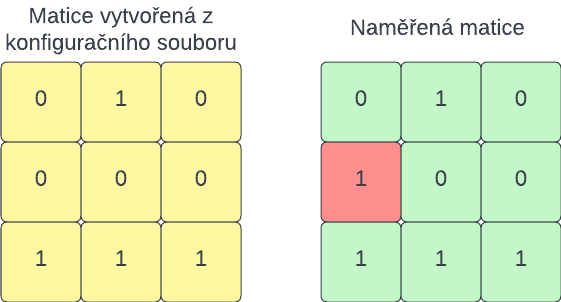
\includegraphics[width = 0.7\textwidth]{obrazky/MATRIX_COMPARISSON.png}
    \caption{PASS/FAIL matrix}
    \label{fig:PASS/FAIL matrix}
\end{figure}

V matici naměřených hodnot jsou zeleně znázorněny výsledky, které se shodují s předpokládanými hodnotami.
Červeně jsou naopak zobrazeny hodnoty, které jsou rozdílné. Hodnota 0 znamená, že mezi externí sondou (probe pinem)
a bRC pinem odpovídající pozici v matici není propojení cesty nižší jak zvolená mezní hodnota odporu.
Naopak hodnota 1 znamená, že mezi sondou a bRC pinem je propojení cesty v požadovaném rozsahu. Z výsledků
měření na obr. \ref{fig:PASS/FAIL matrix} je tedy patrné, že zkoumaný probe pin je někde špatně připojený do 
bRC pinu (řada 2, sloupec 1). Z konfiguračních souborů lze zjistit i název signálu, který vede do tohoto probe
popřípadě bRC pinu a obsluhu informovat o tom, mezi kterými signály a piny vznikl problém.
Tímto postupem se proměří všechny probe piny (každý probe pin má sadu těchto matic).\\


\section{Mód měření přesné hodnoty odporu}
Tento mód se oproti PASS/FAIL módu liší tím, že zde nejsou kladeny žádné nároky na čas měření, protože proces
je plně automatizován a měření probíhá pouze mezi bRC piny.
V tomto módu však tester zjišťuje co nejpřesnější hodnotu propojení cest.
Obdobně jako v PASS/FAIL módu je výsledkem matice propojení, kde jsou nyní však místo jedniček a nul hodnoty
změřeného odporu. Matice vytvořená z konfiguračních dat však zůstává stejná, protože data v sobě nemají
žádné hodnoty odporu propojení. Lze pak stanovit určitý treshold obdobně jako při PASS/FAIL režimu a
určit tak, zda naměřené hodnoty odpovídají očekávaným datům. Následující obrázek ukazuje 
vzniklé matice pro jeden bRC pin pro zvolený treshold 30\,$\Omega$.\\

\begin{figure}[ht!]
    \centering
    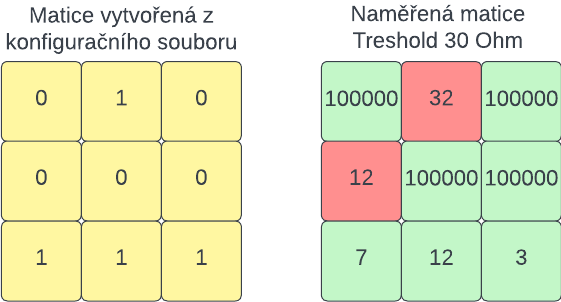
\includegraphics[width = 0.7\textwidth]{obrazky/MATRIX_TRUEVALUE.png}
    \caption{TRUEVALUE matrix}
    \label{fig:TRUEVALUE matrix}
\end{figure}

V obr. \ref{fig:TRUEVALUE matrix} lze najít hodnoty odporu 100000$\Omega$. Tyto hodnoty však neodpovídjí reálné hodnotě propojení
cest, ale je značí že měřená hodnota odporu je mimo rozsah testeru a lze tak předpokládat, že zde žádné propojení není.
Dále je zde možno najít červené pole s hodnotou 32$\Omega$. Podle matice vytvořené z konfiguračního 
souboru by tato cesta měla být propojená. Nicméně pro zvolený treshold 30$\Omega$ je tato hodnota odporu propojení
považována za příliš vysokou a vyhodnocena jako chybné propojení.\\

Přesná hodnota odporu se zde měří tak, že pro každou skupinku pinů, je vytvořena rampa D/A převodníku a 
monitoruje se, při jaké hodnotě napětí na D/A převodníku se překlopí výstup komparátoru daného pinu. Aby se 
minimalizovala chyba vzniklá úbytkem napětí na P-channel mosfetu (viz kapitola o návrhu měřící karty),
lze zároveň využít rampu D/A převodníku pro změření přesného výstupu napětí bRC pinu a výsledek měření tak vztáhnout
přímo k napětí na bRC pinu.\\

\chapter{Řídící PC aplikace}
Pro účely testeru byla vyvinuta PC aplikace založená na programovacím jazyku python. Tato aplikace umožňuje
nejen komunikovat s testerem a provádět měření, ale také převádět vstupní CAD, CAM, gerber a různé textové konfigurační
soubory do vhodného formátu pro účely testeru.\\

Aplikace se skládá ze 3 hlavních záložek (Routing, Probe Test a Auto Test) v horním levém rohu. V semestrální práci Je
dokončena funkce pouze záložky routing.

\section{Záložka routing}
Tato část řídící aplikace má na starosti převod všech vstupních dat do vhodného grafického zobrazení a vytvoření
propojovacích matic (viz obr. \ref{fig:TRUEVALUE matrix} a Obr.\ref{fig:PASS/FAIL matrix}).
Ve svém GUI je záložka koncipována tak, aby obsluha testu byla schopna identifikovat různá propojení bRC a probe pinů.
Zároveň by mělo být možné na základě tohoto GUI zapojit celou fixture část.\\

\begin{figure}[ht!]
    \centering
    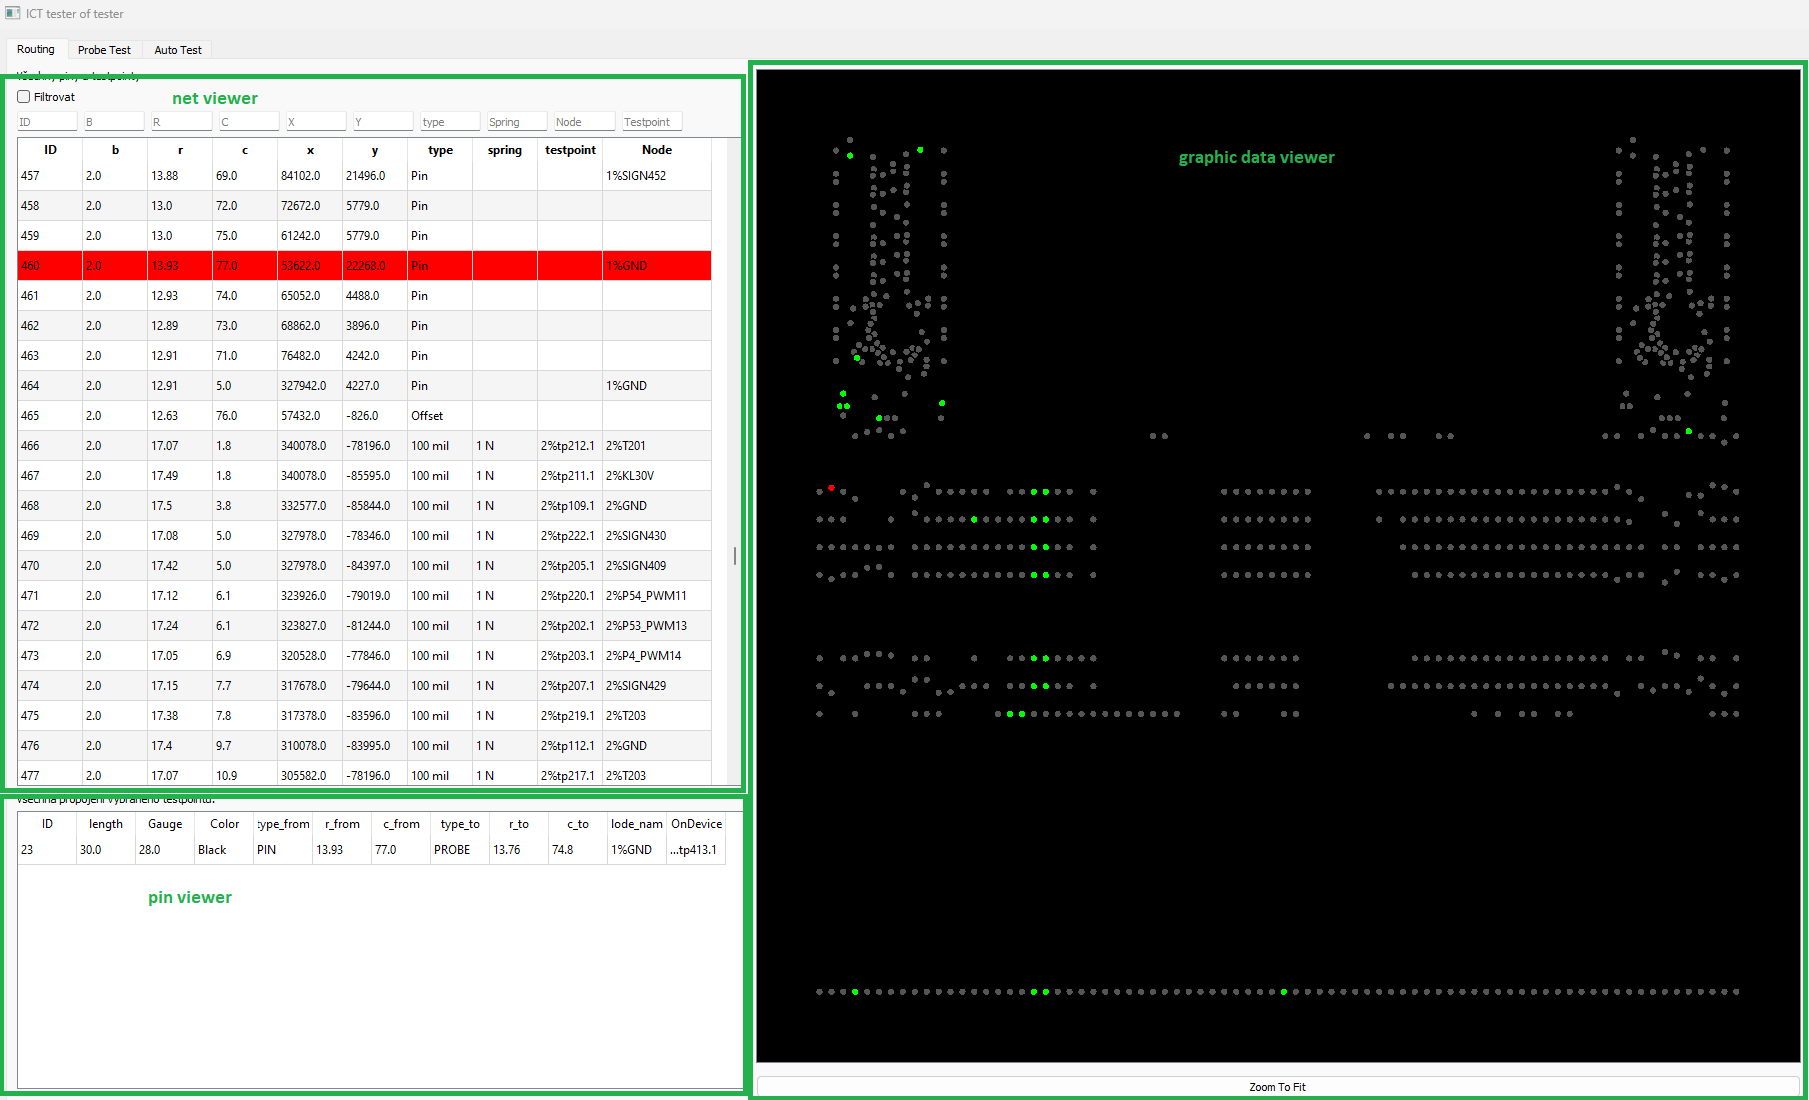
\includegraphics[width = 1\textwidth]{obrazky/PC_AP_top_view.png}
    \caption{PC aplikace - záložka routing}
    \label{PC aplikace - záložka routing}
\end{figure}

Záložka se skládá ze 3 hlavních částí (net viewer, pin viewer a data graphics viewer).
V části netviewer jsou zobrazeny všechny bRC a probe piny (jsou zde i jiné piny, které nejsou diskutovány v diplomové práci).
Každý pin zde má svou polohu vyjádřenou dvěma způsoby. Prvním způsobem je značení pomocí bRC. Toto označení je
vztaženo k mřížce, kterou tvoří spodní část fixture (obr. \ref{fig:ICT_tester}). Protože jednotlivé piny mají svou toleranci
a nemusí ležet přímo v bodě mřížky, je označení bRC nepřesné a je zaokrouhleno k nejbližšímu bodu mřížky.
Druhým a přesným způsobem je označení pomocí x a y souřadnic.\\

Některé piny mají neprázdná pole označení ve sloupci testpoint.
Toto označení znamená, že se jedná o probe pin a bude ho nutné otestovat externí sondou. Zároveň probe piny
mají ve sloupci type průměr testovací jehly (bRC piny mají označení pin). Dále je zde vidět Node (uzel) do kterého pin patří.\\

Po kliknutí do příslušného řádku v části netviewer se v části graphic data viewer zobrazí červeně zvolený pin
a zároveň zeleně všechny probe a bRC piny se stejným označením node (obr. \ref{PC aplikace - záložka routing}).
V části graphic data viewer zároveň lze klikat myší na jednotlivé piny a tím je označit v sekci netviewer.
Takto lze jednoduše procházet zapojení fixture části. Část graphic data viewer umožňuje různě přibližovat a posouvat
zobrazení.\\

V části pin viewer jsou zobrazeny podrobné informace o vybraném (červeném) pinu.
Každý řádek v této sekci (může jich být libovolný počet) obsahuje informace o propojení zvoleného červeného pinu s nějakým
dalším pinem. Na obr(\ref{PC aplikace - záložka routing}) je patrné, že v části pin viewer je pouze jeden řádek, ale zároveň
z části graphic data viewer je jasně vidět, že uzel 1\%GND obsahuje daleko více pinů. To je způsobeno tím,
že uzly nejsou vždy tvořeny paralelním propojením všech pinů. Dále aby bylo možno fixture zapojit, obsluha musí v části
pin viewer vidět pouze propojení kam dále má vést propojení. Zobrazeny jsou tedy pouze cesty, které vedou z tohoto pinu.
Toto je patrné i z informací v příslušném řádku části pin viewer. V obr.(\ref{PC aplikace - záložka routing}) jsou ve sloupcích
r\_from a c\_from (značí z kterého pinu vede cesta) stejná data jako ve sloupcích r a c v části netviewer. Jedná se tudíž
o červený vybraný pin. Sloupce r\_to a c\_to jsou souřadnice pinu, kam má vést další cesta. Po kliknutí do řádku
v části pin viewer se v části graphic viewer znázorní pomyslné propojení (\ref{PC aplikace - Zobrazení cesty}).
Zároveň lze z řádku v sekci pin viewer vyčíst data o délce, typu a barvě použitého propojovacího drátu.
\begin{figure}[ht!]
    \centering
    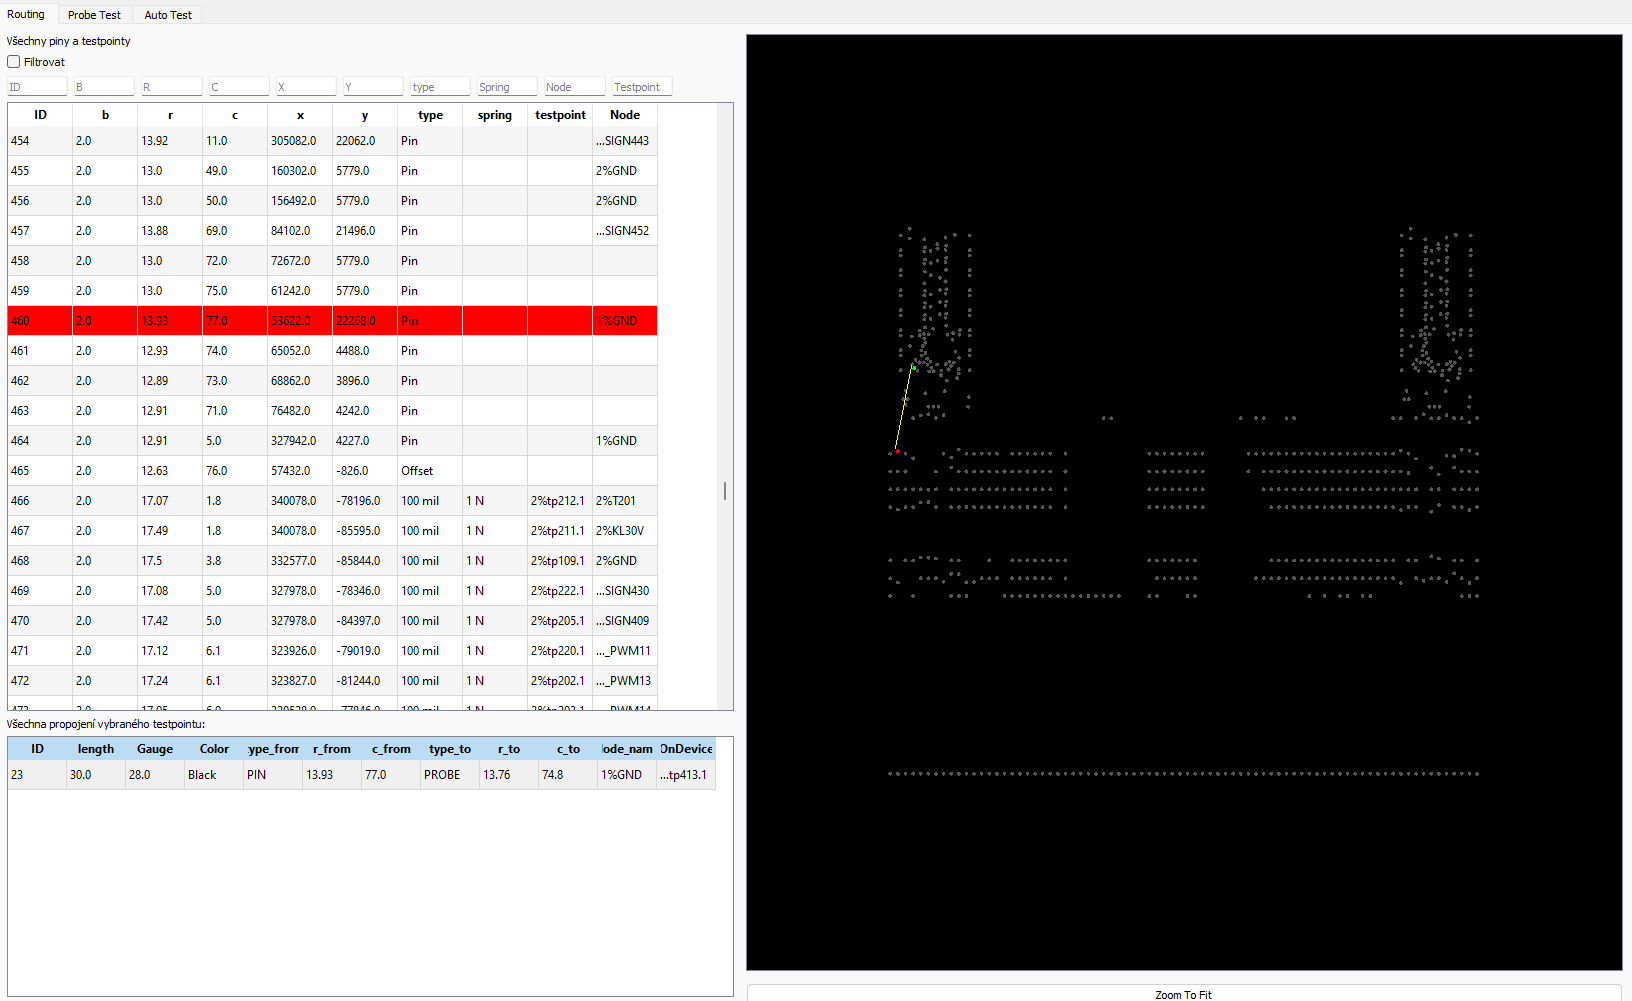
\includegraphics[width = 0.9\textwidth]{obrazky/PC_AP_top_only1.png}
    \caption{PC aplikace - Zobrazení cesty}
    \label{PC aplikace - Zobrazení cesty}
\end{figure}